 \section{实验结果与分析}

\subsection{Phoenix较差scalability的实验结果}
实验结果显示\ref{phoenix:speedup},
8核以上,随着核数的增多,Phoenix的性能越来越差,
其中hist表现的最为明显,
通过详细分析发现,
hist中有几个被频繁访问的全局变量分别为:
red\_keys[256],blue\_keys[256],green\_keys[256];
多个map线程会并发地访问这些全局变量,
{\color{gray}(这会导致多个线程竞争Linux中保护进程描述副的读写信号量,
这个读写信号量是用来保证同一个进程创建的多个线程串行地访
问同一个进程的描述符。)}(需要继续补充和验证的)
通过收集perf record的数据\ref{phoenix:spinlock},
结果显示,随着核数的增多,ticket\_spin\_lock的开销越来越大,
并且在16和32核下,它们是最耗时的函数,
分别占整个程序开销的 40.50\%和 71.25\%。
虽然lr, sm, wc, pca中没有频繁访问的全局变量,
但是Phoenix是基于Pthread多线程编程的,
随着核数的增多,多个线程需要竞争内核态锁和信号量,
导致ticket\_spin\_lock过高。

此外,我们发现使用不同的内存分配器也会影响应用程序的性能.
通过对比Phoenix-jemalloc和Phoenix-glibc的时间,
可以发现,
hist, wc, pca在高核下Phoenix-jemalloc性能较好。
因此,在高核数环境下,Phoenix使用相对稳定的jemalloc,
具有更好的性能\ref{phoenix:diff_malloc}。
\begin{figure}[!h!t]  
    \centering
    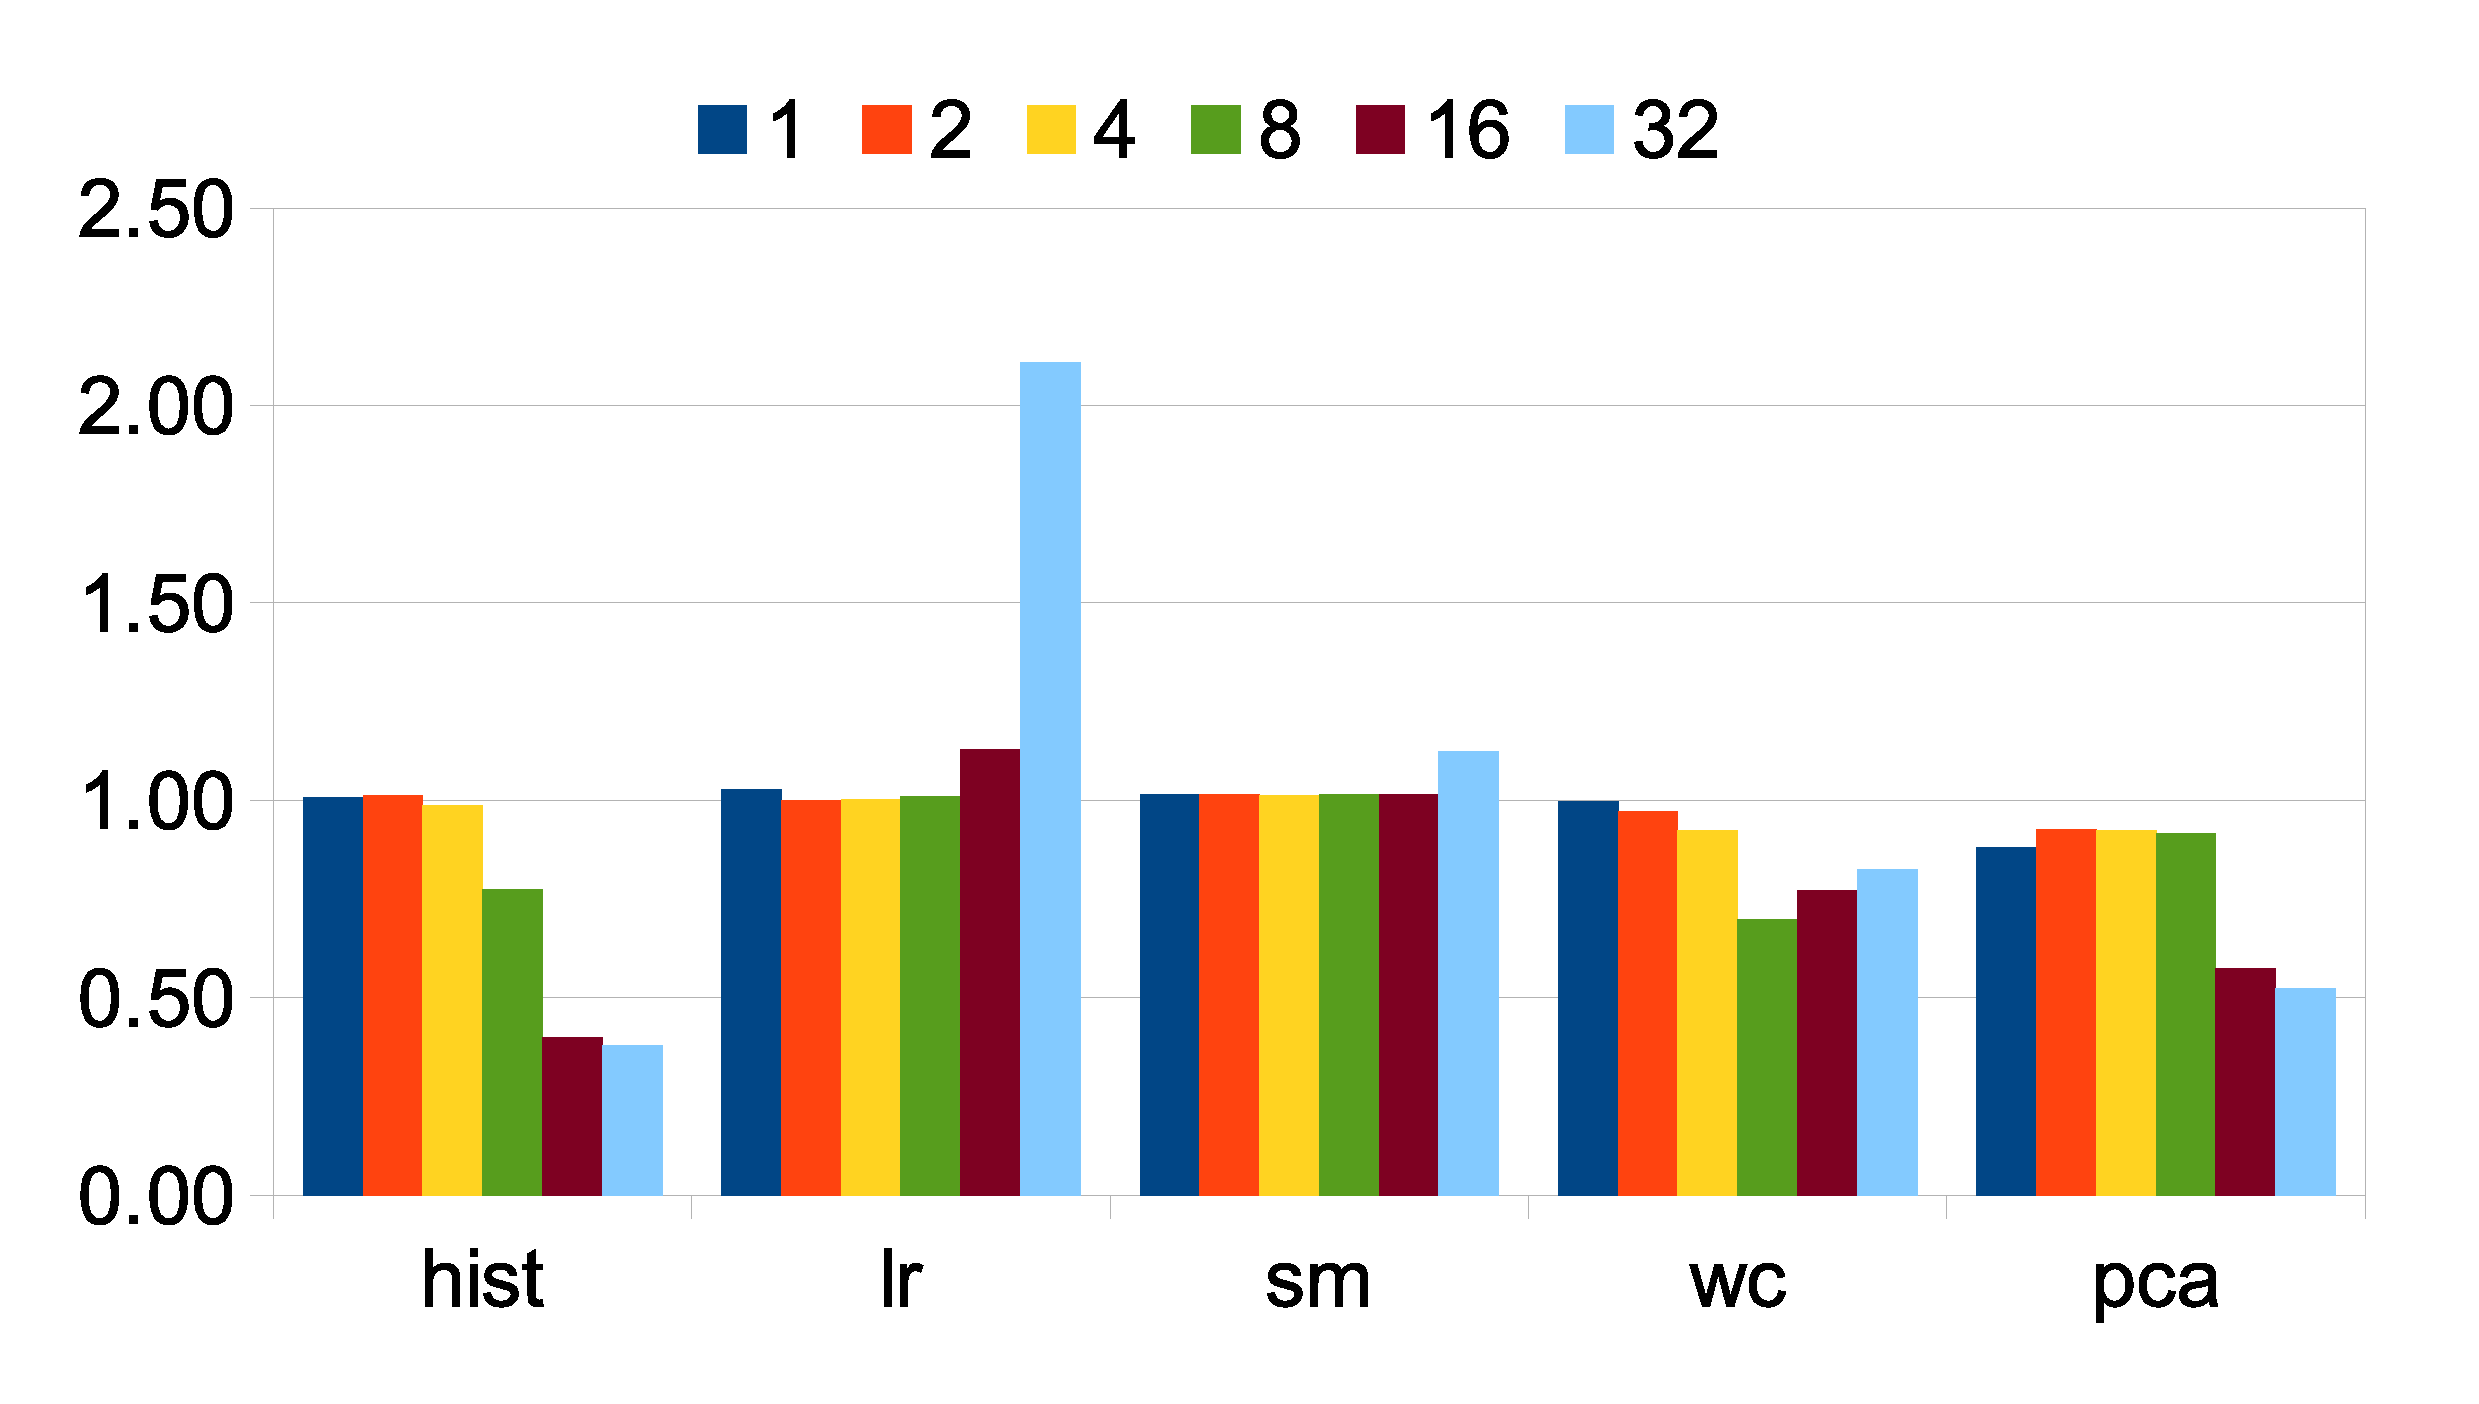
\includegraphics[width=0.45\textwidth]{img/phoenix_diff_malloc.eps}
    \caption{Phoenix-jemalloc / Phoenix-glibc no combiner}
    \label{phoenix:diff_malloc}
\end{figure}

然而,即使Phoenix-jemalloc具有较好的性能,
其scalability也是较差的,如图\ref{phoenix:jemalloc_no_comb_speedup},
\begin{figure}[!h!t]  
    \centering
    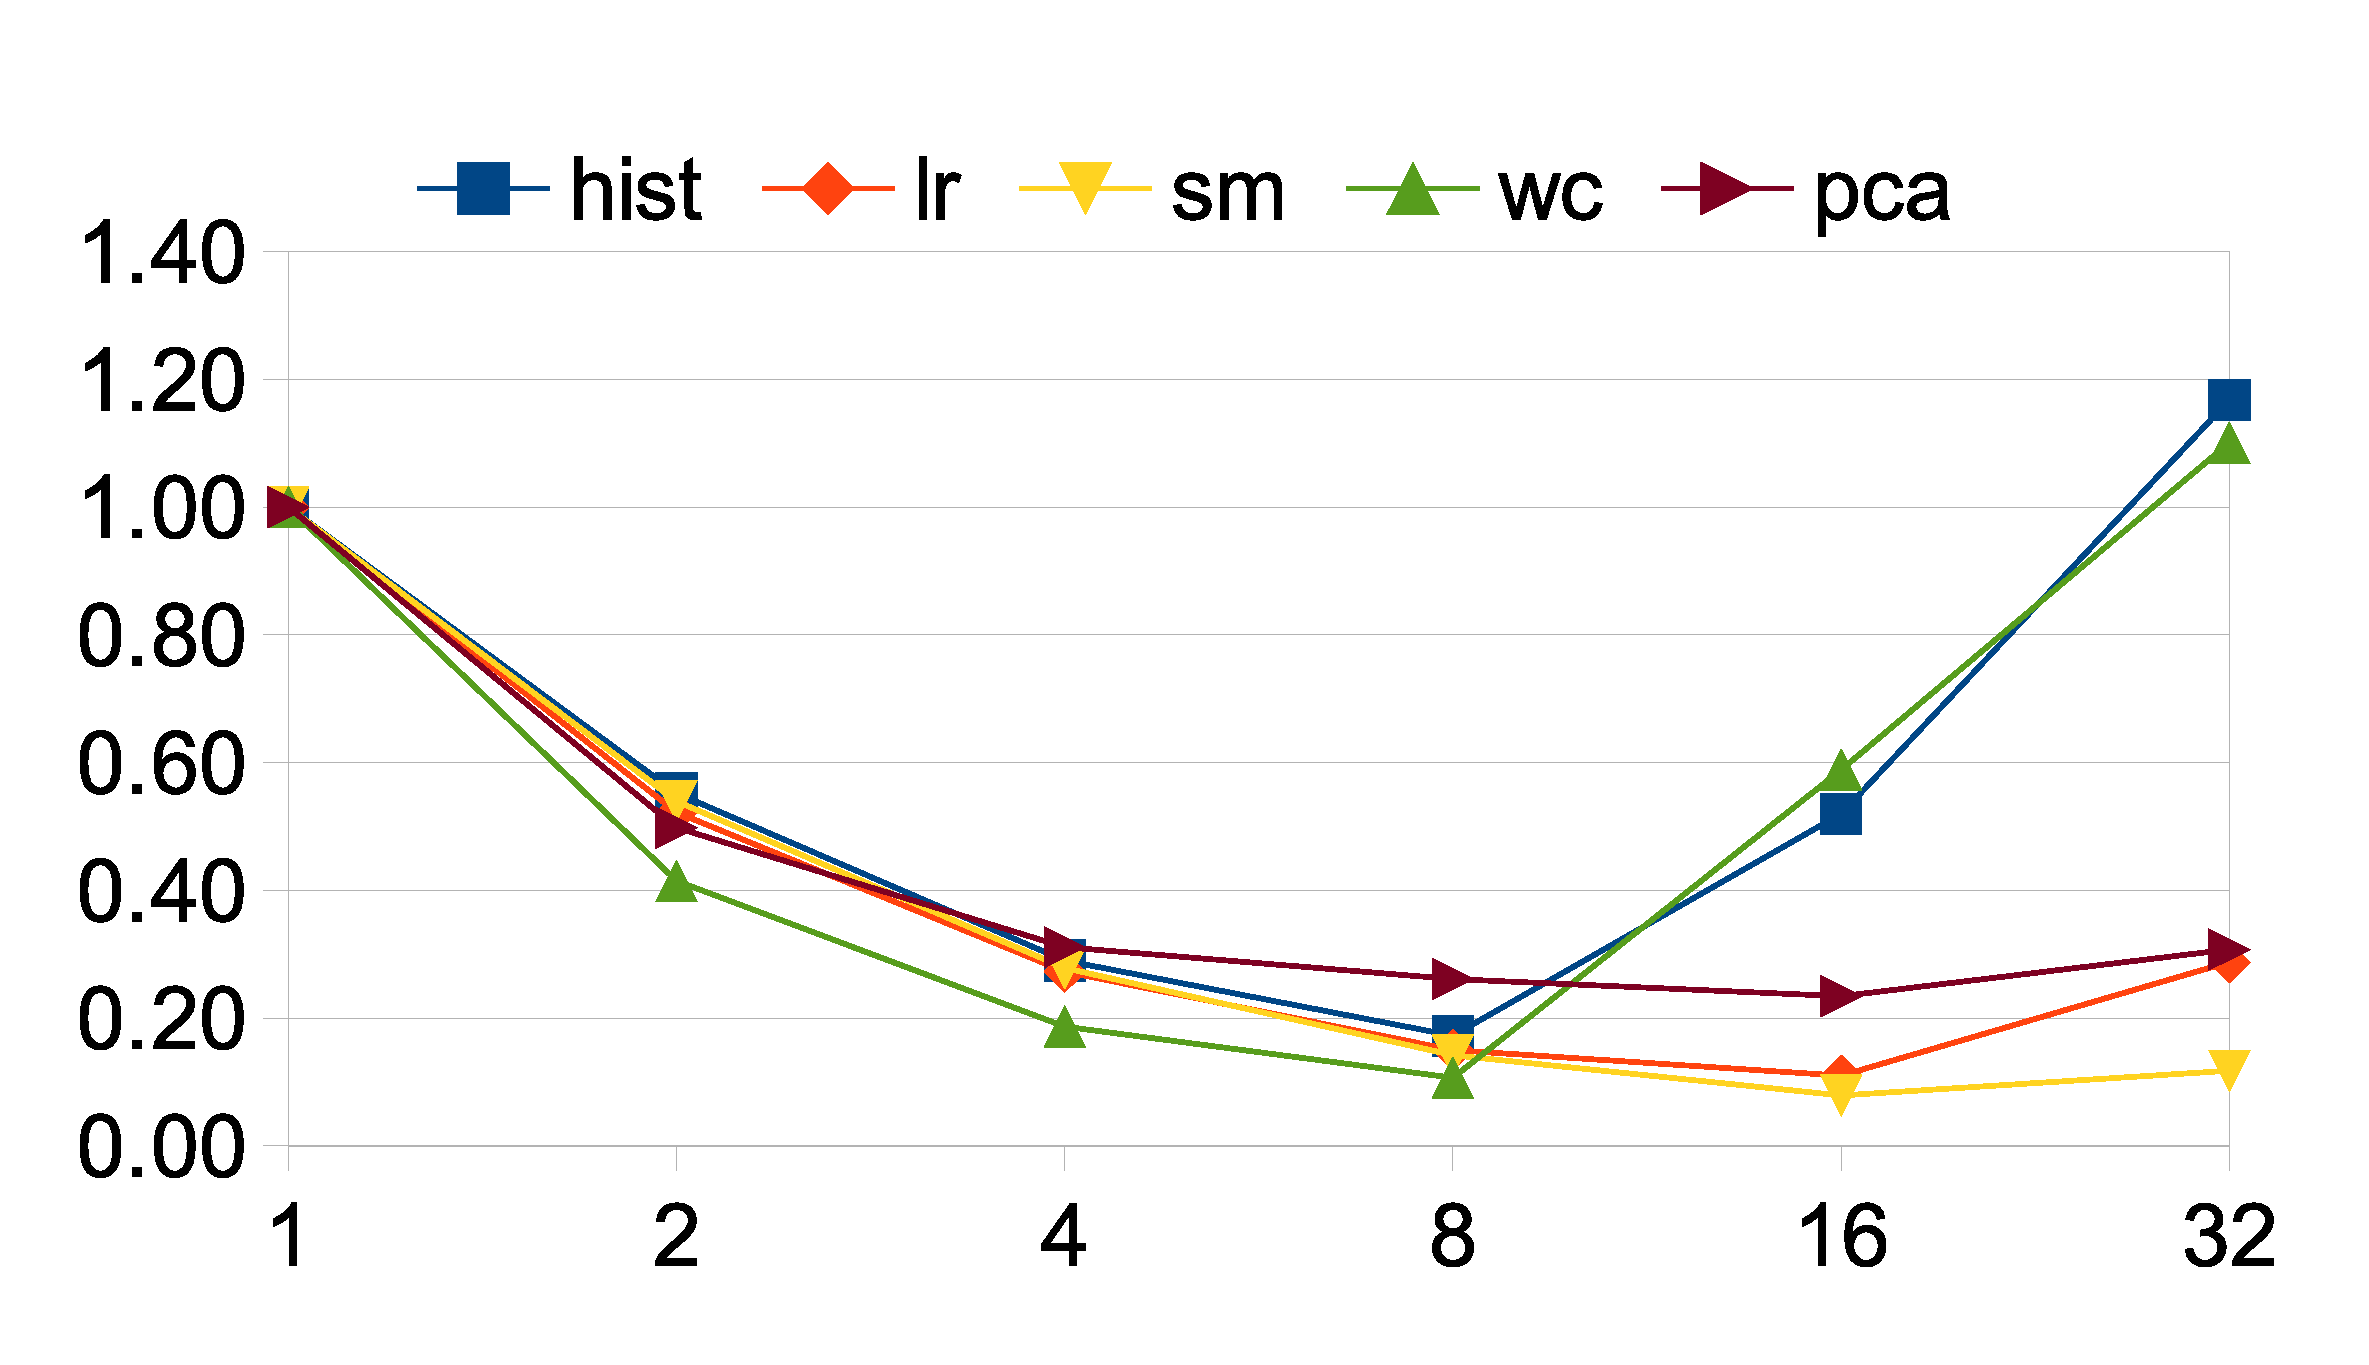
\includegraphics[width=0.45\textwidth]{img/phoenix_jemalloc_no_comb_speedup.eps}
    \caption{Phoenix jemalloc no combine speedup}
    \label{phoenix:jemalloc_no_comb_speedup}
\end{figure}
我们可以看出,wc,hist在8核以上,性能越来越差;
通过perf record的详细分析发现,
相比Phoenix-glibc,
Phoenix-jemalloc的ticket\_spin\_lock明显降低,
但随着核数的增多,该部分的开销也是越来越大,
特别地,在16核与32核情况下,
wc的ticket\_spin\_lock的开销分别为24.04\%和39.91\%。

将具有较好性能的Phoenix-jemalloc与DMR进行对比,
实验结果如图\ref{dmr:time_jemalloc}所示,
\begin{figure}[!h!t]  
    \centering
    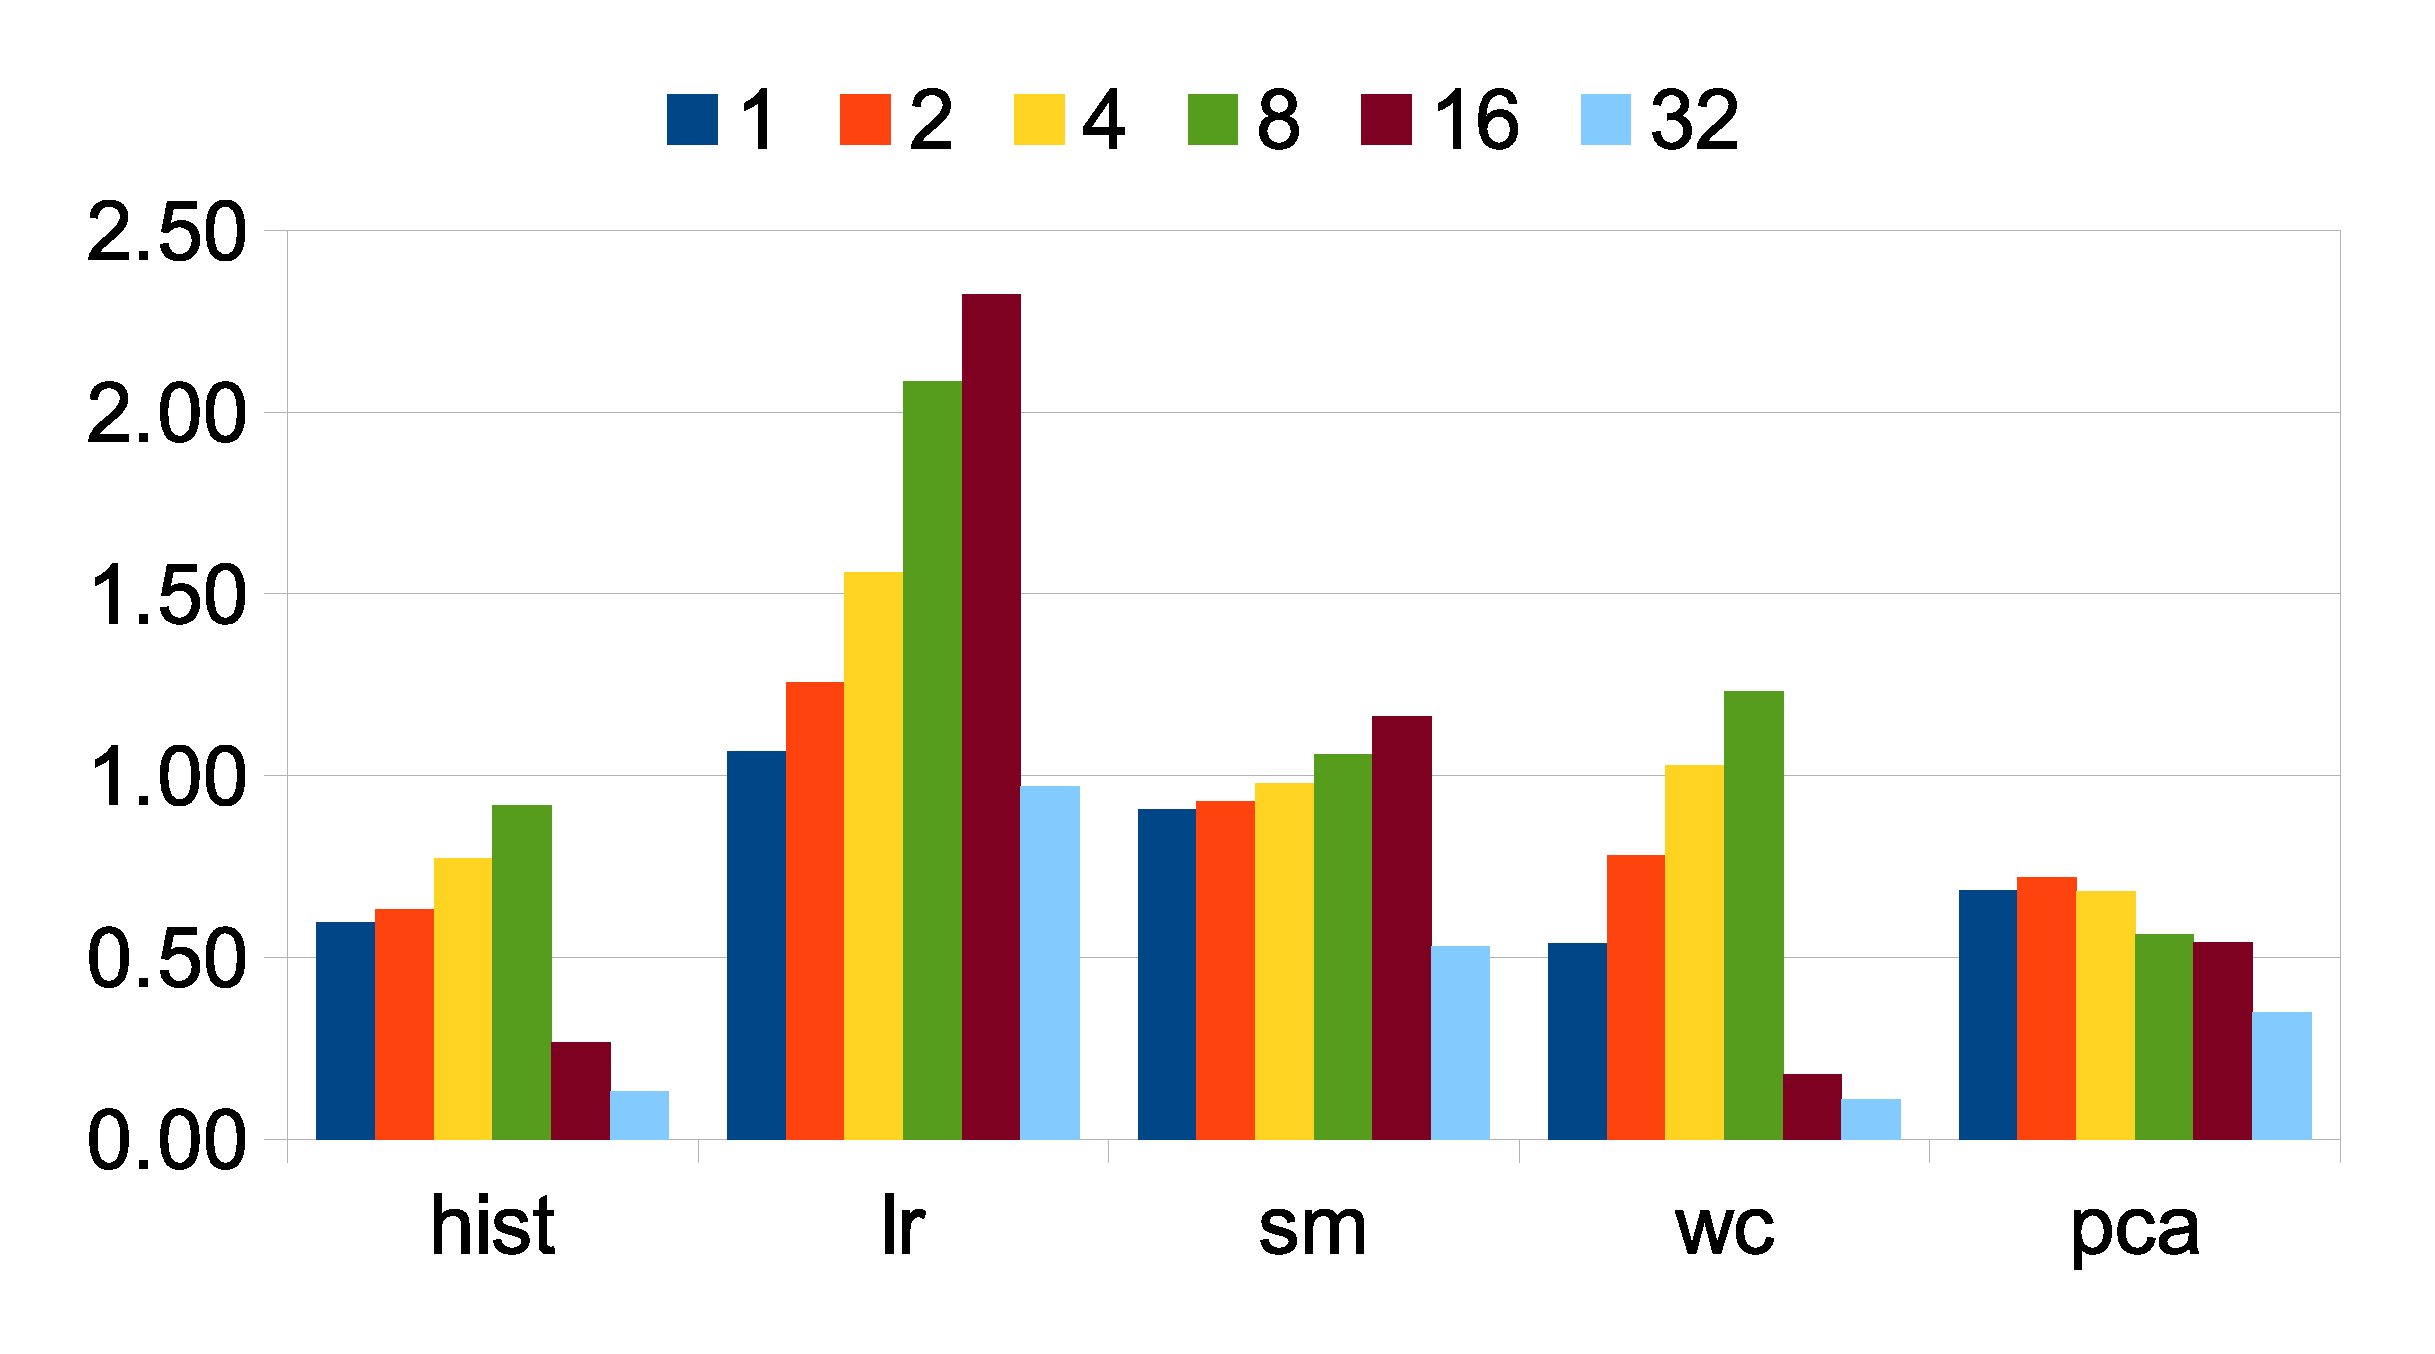
\includegraphics[width=0.45\textwidth]{img/dmr_time_jemalloc.eps}
    \caption{DMR-array / Phoenix-jemalloc no combine}
    \label{dmr:time_jemalloc}
\end{figure}
可以看出,除了lr,DMR表现的性能都较好,
特别地,在16和32核情况下,DMR的性能远优于Phoenix-jemalloc。
结合DMR和Phoenix-jemalloc的scalability,
我们可以推测,在高核情况下,
核数越多,DMR的优势会更加明显。


\subsection{piepeline带来的性能优势}
开启单线程情况下,可以看出pipeline带来的性能优势,


\subsection{DMR环境初始化的开销分析}
DMR采用新的Producer-Consumer模型,
以及地址空间隔离的进程,
它为DMR带来好的性能的同时,
也存在一部分额外的开销,
主要表现在环境初始化部分。
环境初始化的时间主要是指:
从应用程序调用mapreduce库开始,到Map阶段开始前的时间。

Phoenix环境初始化主要包括:
全局变量的构建和初始化,
map任务队列的初始化,
thread pool的创建和初始化
(包括构造thread pool需要的控制结构、线程的创建、启动线程);
DMR环境初始化中全局变量和map任务队列的初始化与Phoenix相当,
主要差别在于producer-consumer模型的搭建,
它包括进程的创建、producer和consumer角色的设置、
map worker和reduce worker之间一对一的隐式queue的构建,
实验结果显示该部分的开销远大于Phoenix中thread pool的创建。
\begin{figure}[!h!t]  
    \centering
    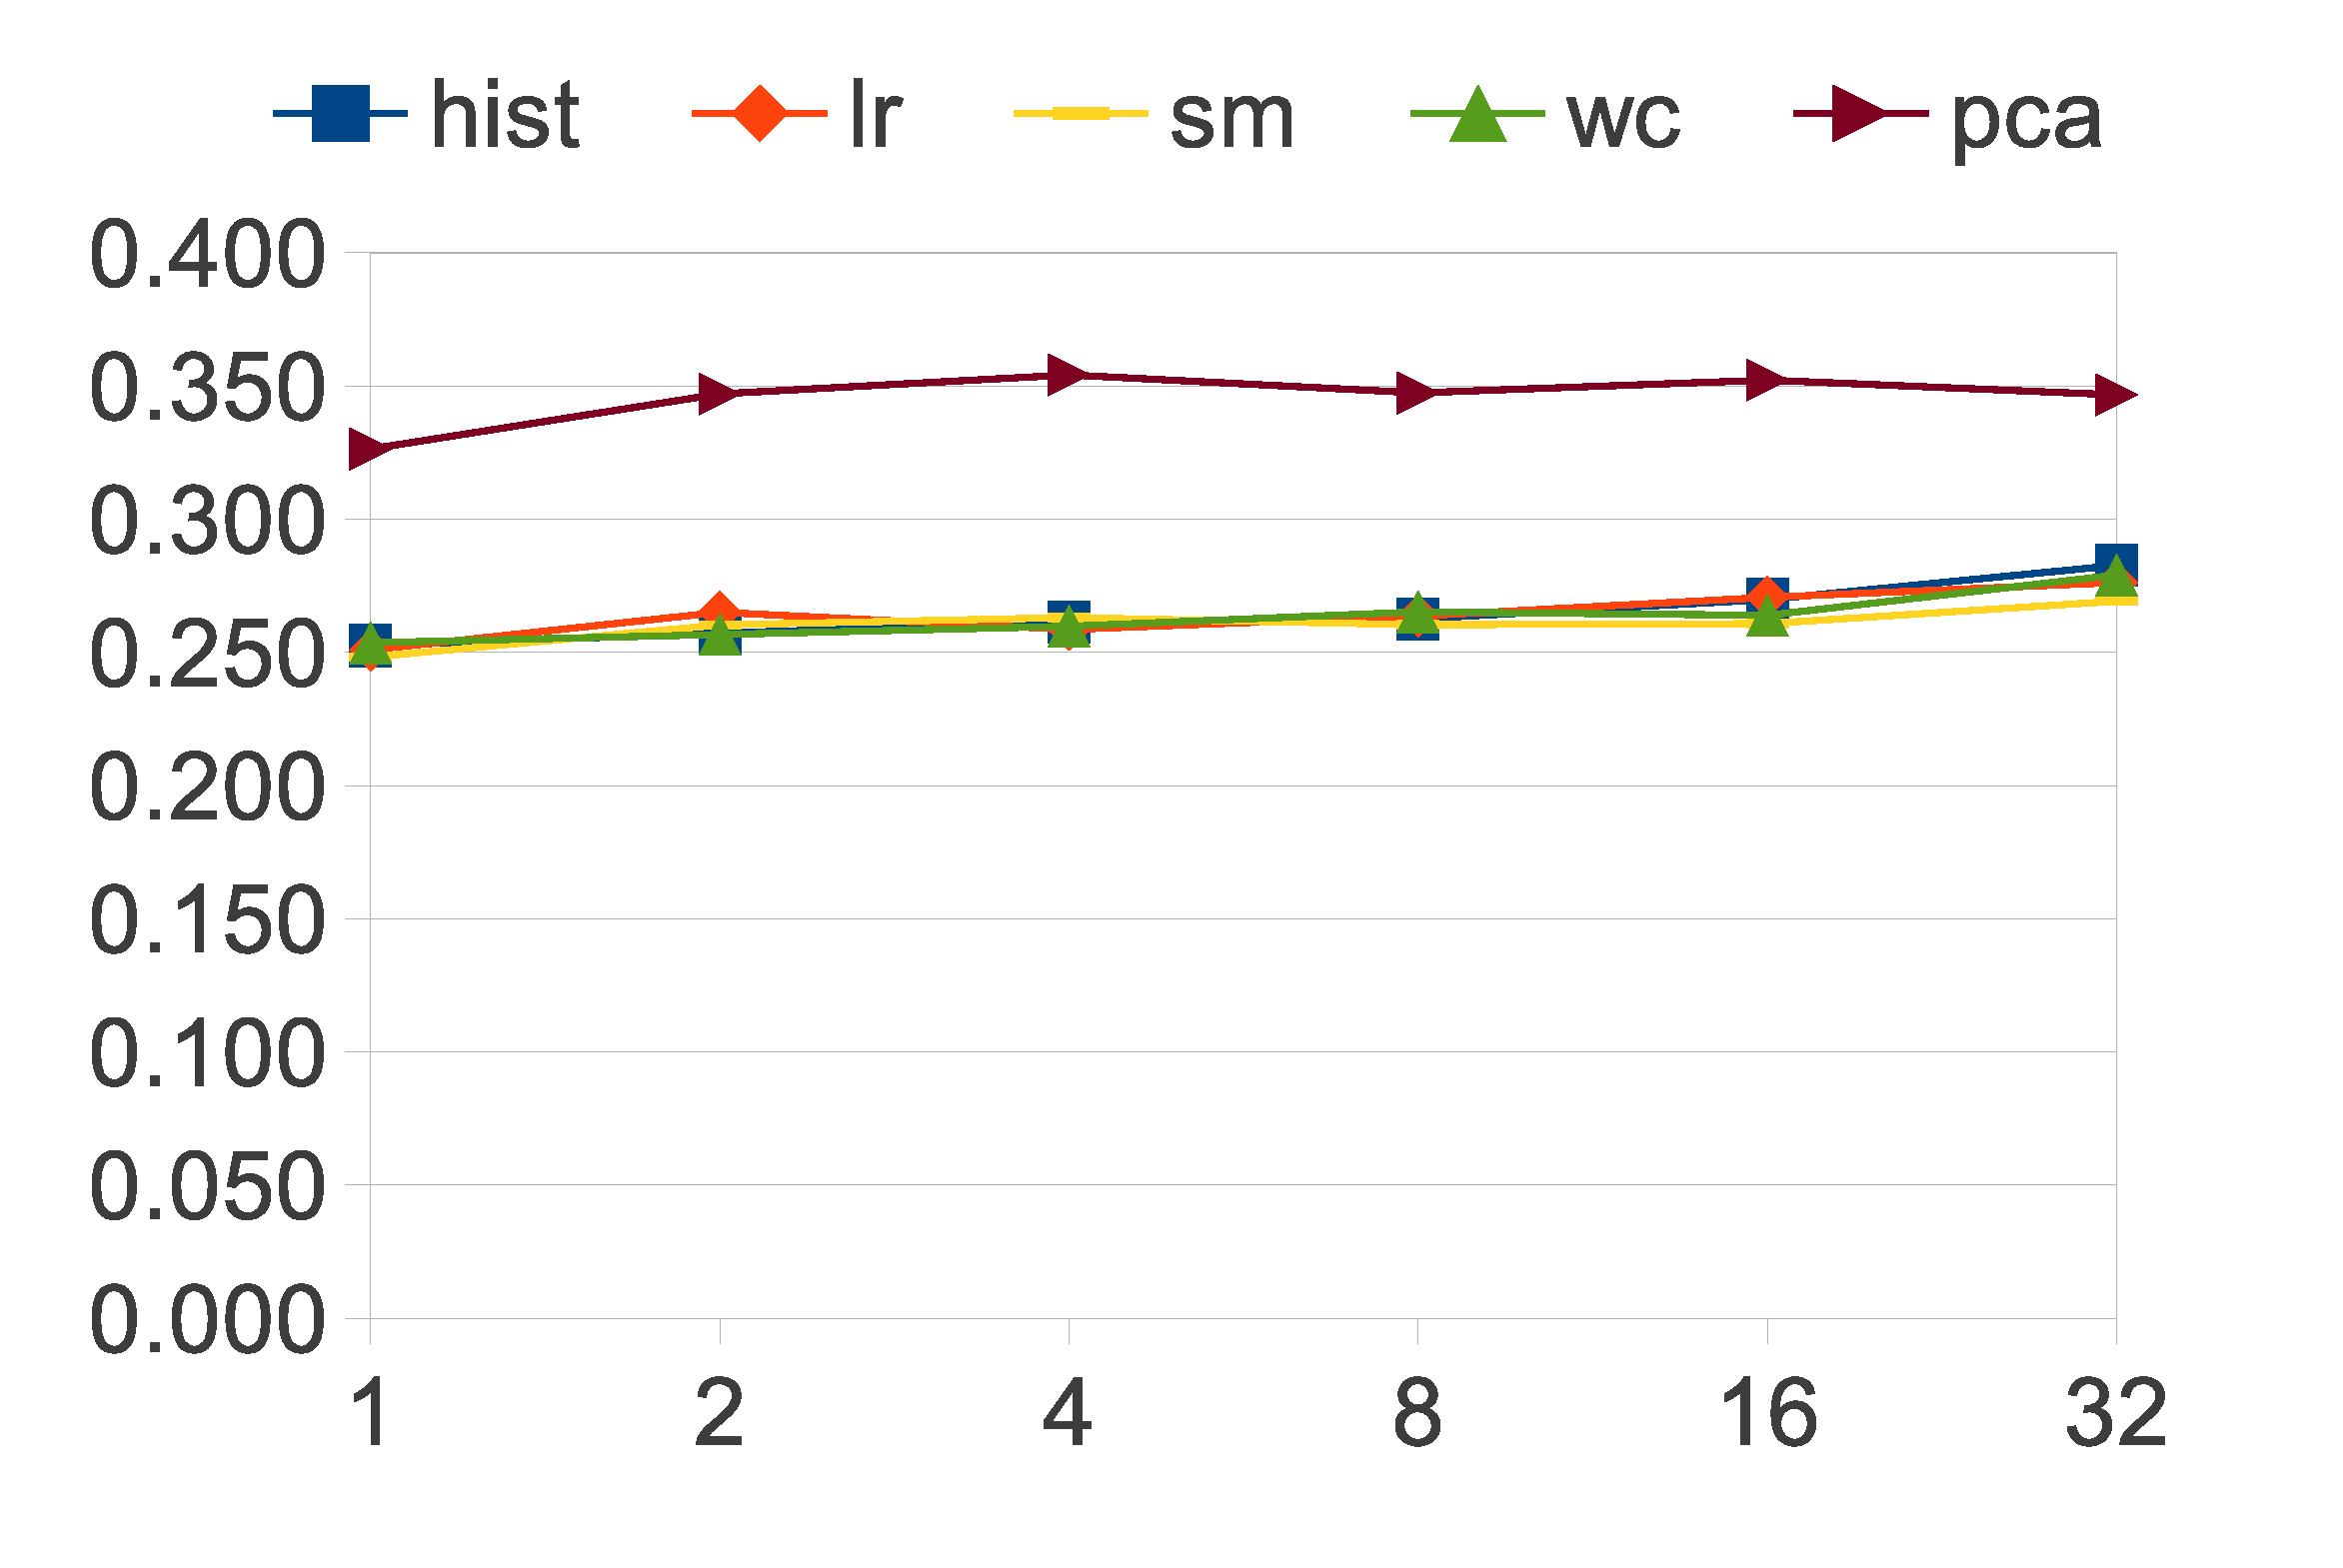
\includegraphics[width=0.45\textwidth]{img/dmr_spmcinit.eps}
    \caption{DMR environment initialize time(seconds)}
    \label{dmr:environment}
\end{figure}
\begin{figure}[!h!t]  
    \centering
    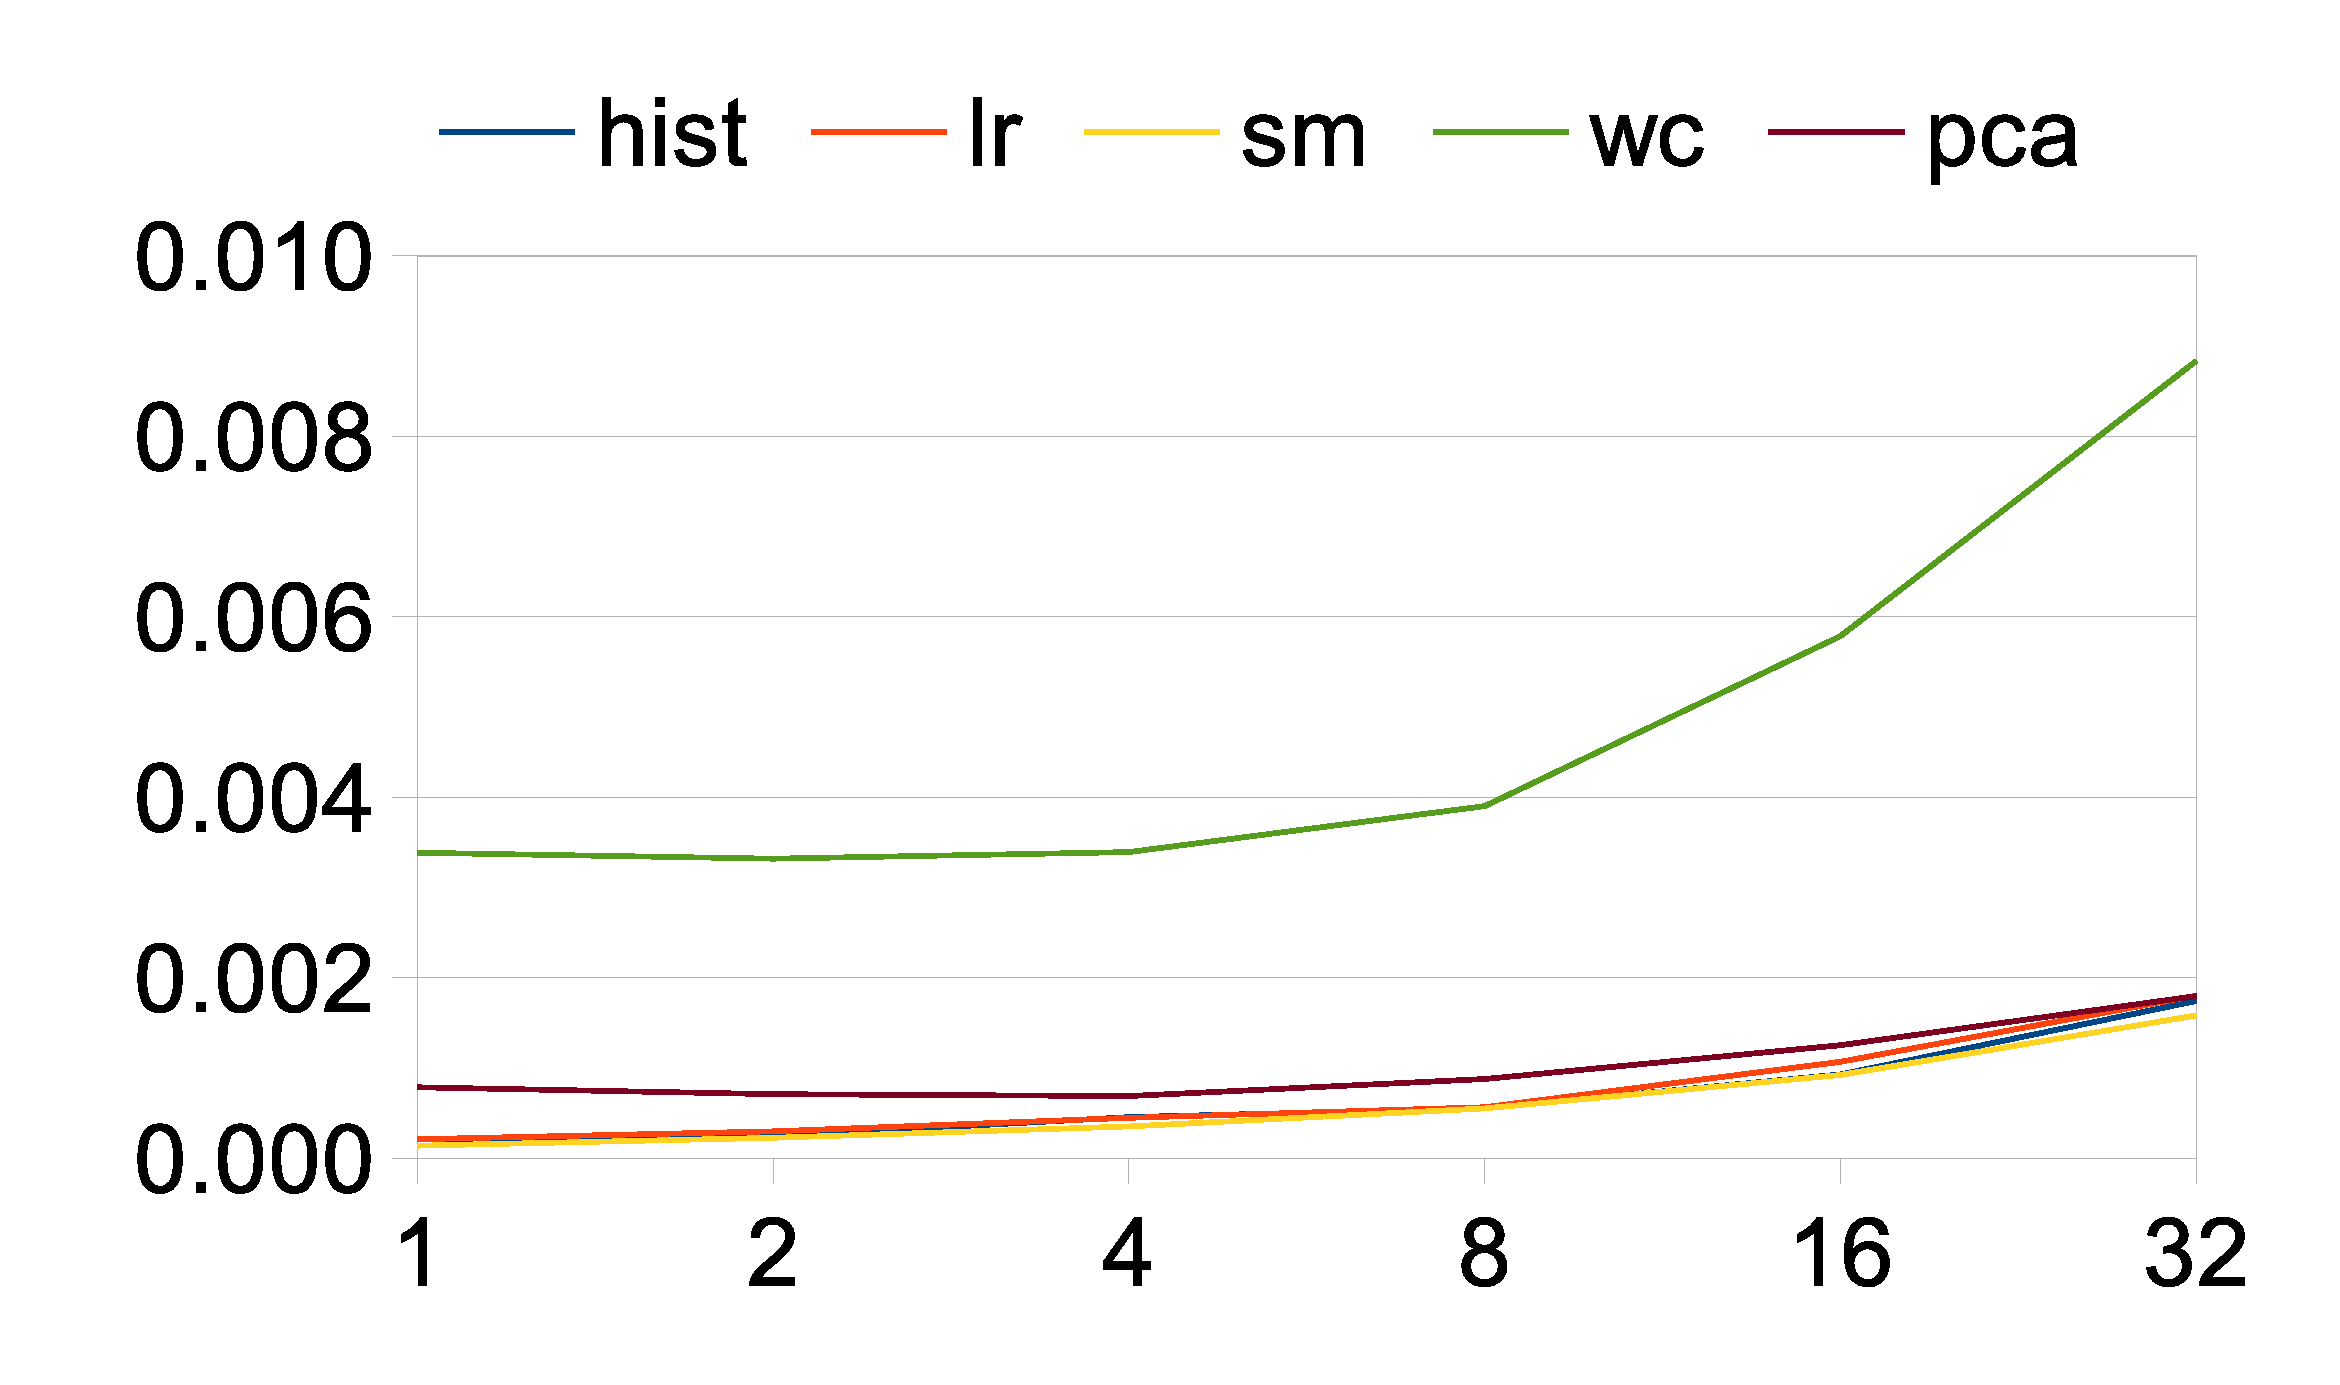
\includegraphics[width=0.45\textwidth]{img/phoenix_init.eps}
    \caption{Phoenix environment initialize time(seconds)}
    \label{phoenix:environment}
\end{figure}

如图\ref{dmr:environment}所示,
DMR初始化时间为0.25s~0.35s,
Phoenix初始化的时间为0.0002s~0.0020s(如图\ref{phoenix:environment}),
相比之下,DMR初始化花费时间远大于Phoenix。
此外,从数据中我们可以看出,
对不同的应用,不同的核数,
DMR的初始化时间基本稳定,
由此我们可以得出:
针对数据集较大,运行时间较长的应用程序,
初始化时间所占的比例就越小,
DMR的性能就会越好。


图\ref{dmr:time-array}给出了DMR的性能,
其中hist, wc, pca具有较好的性能,
sm持平,lr的性能较差,图\ref{dmr:init-percent}
给出各应用程序初始化时间的占总运行时间的百分比,
可以看出lr的初始化时间所占的百分比相当大,
且高于其他应用程序,
这使得lr在DMR上执行的效率比Phoenix差。

\begin{figure}[!h!t]  
    \centering
    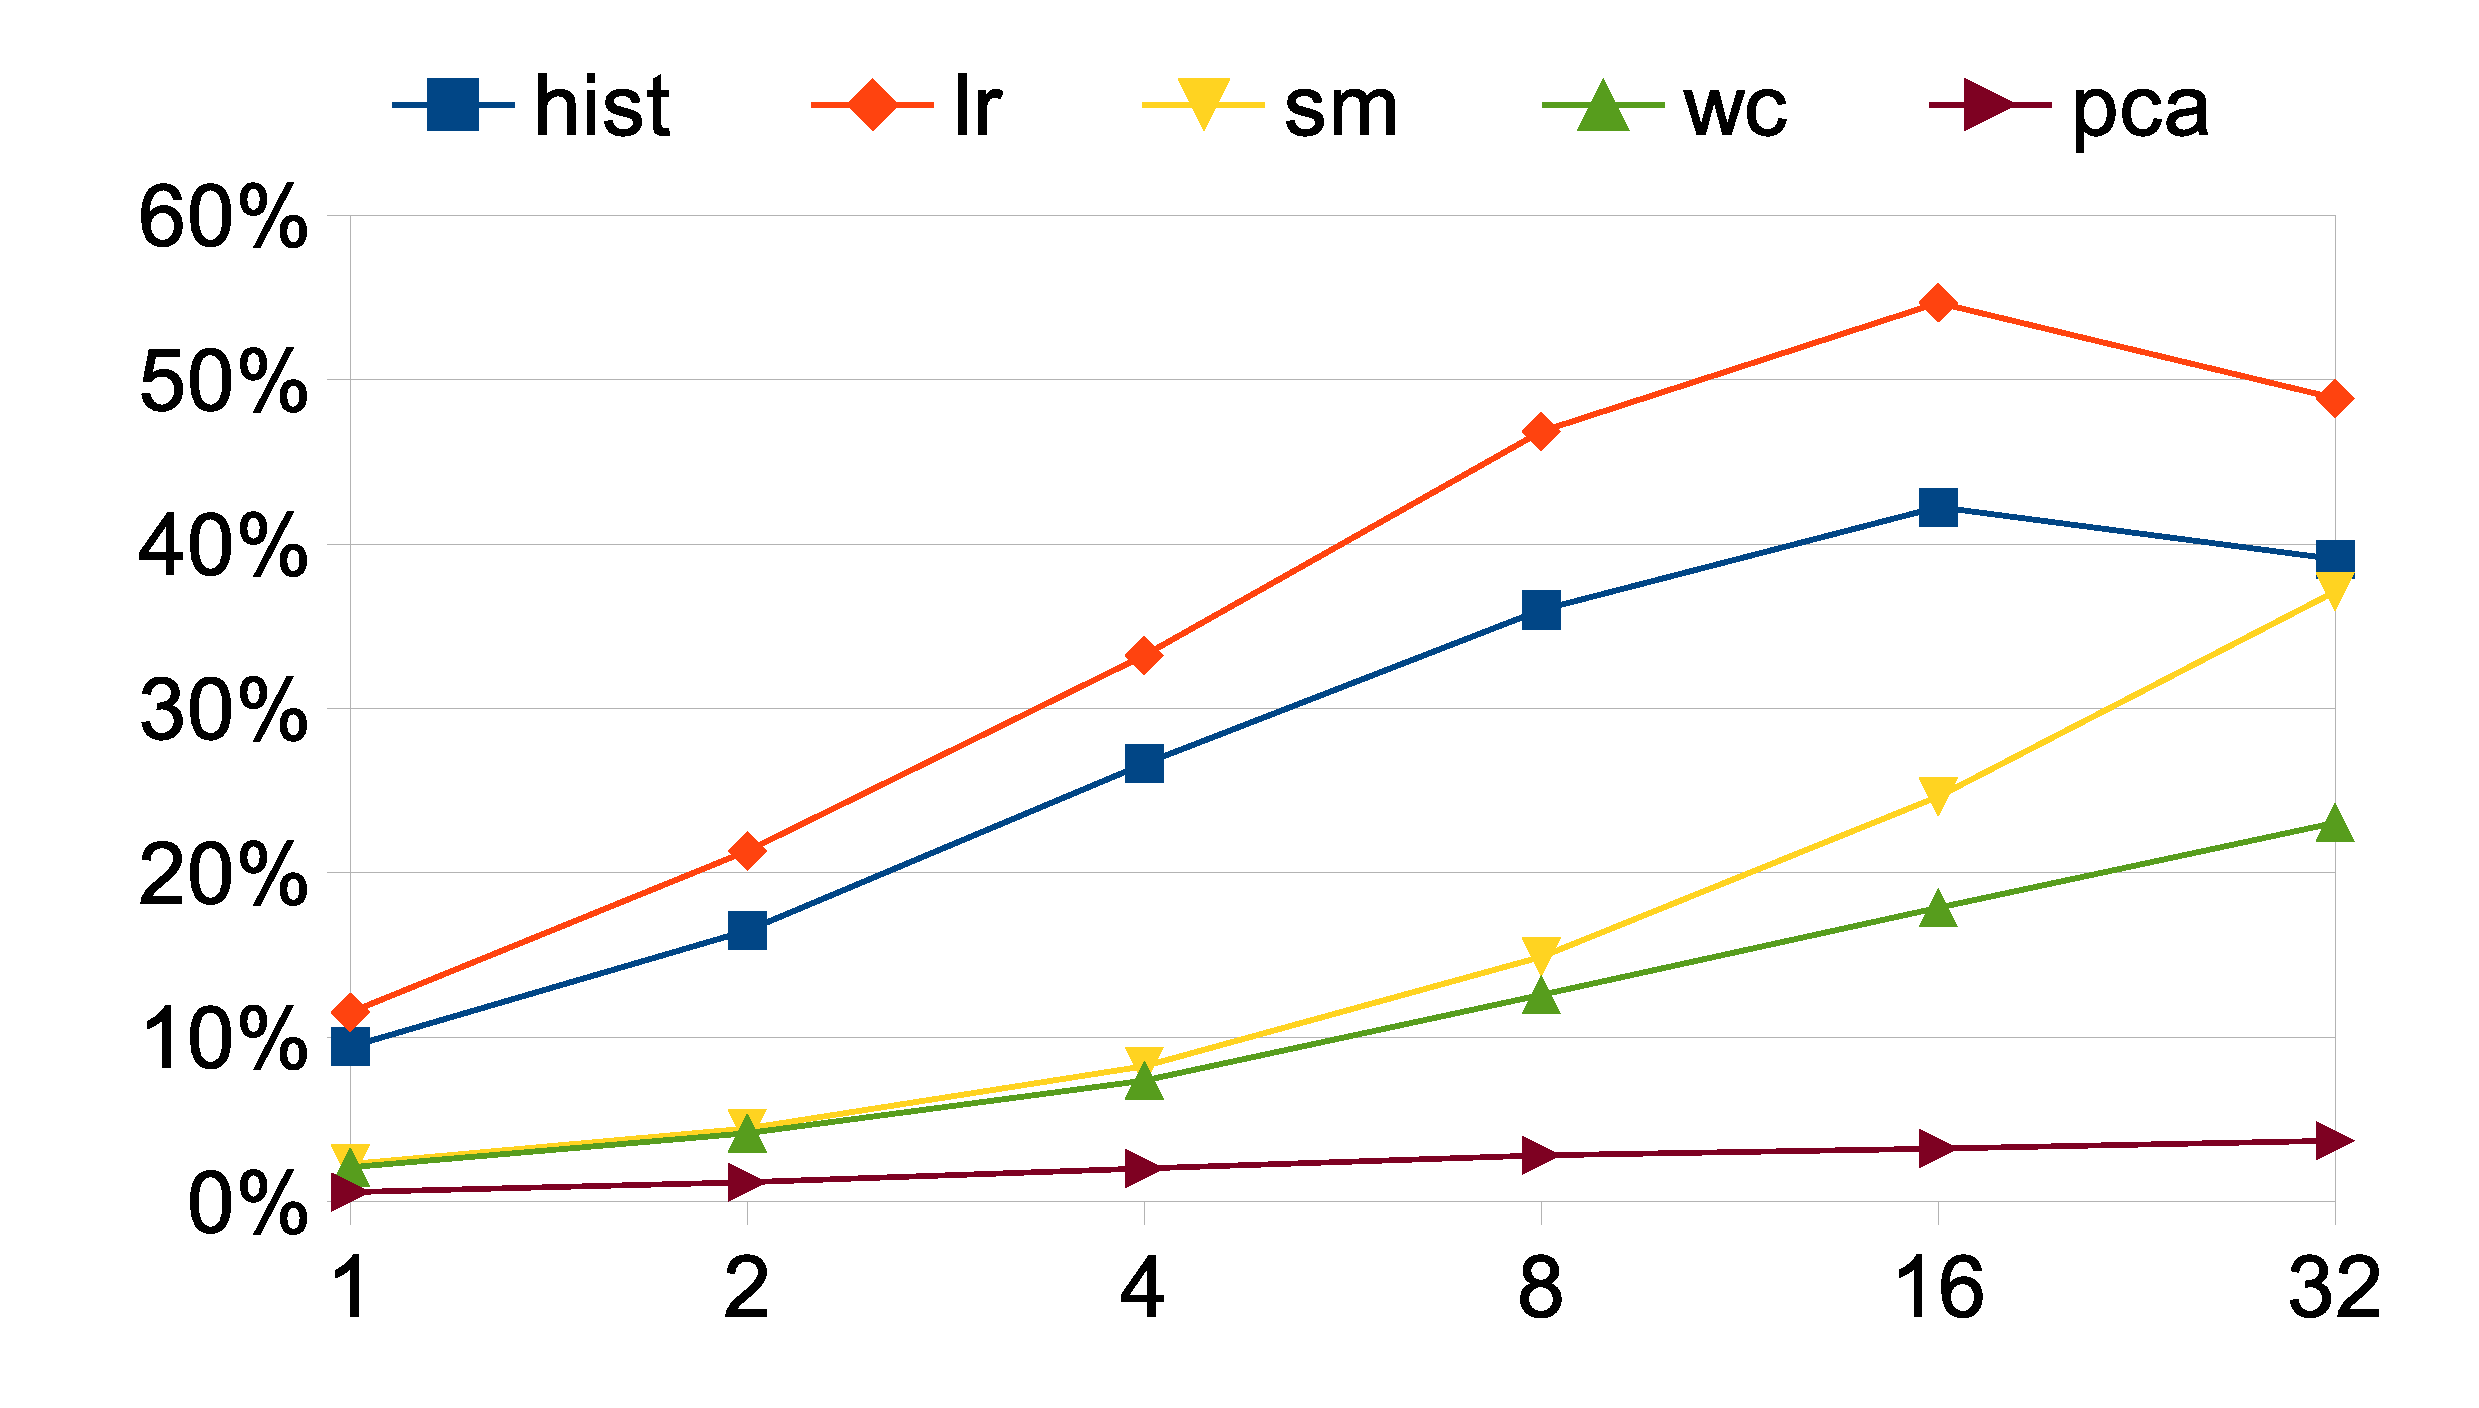
\includegraphics[width=0.5\textwidth]{img/dmr_init_percent.eps}
    \caption{环境初始化时间所占时间的百分比}
    \label{dmr:init-percent}
\end{figure}
\input app 
\input config

\section{附加}
\input twin_diff
\input tstat
